% 16-10-26.tex — V-SIL visual brief: general architecture, Gate G0, Gate G1 (Ctx 02 design)
% Sources: methodology/V-SIL/V-SIL.tex (Figs. 1-2), methodology/V-SIL-v2/G1_DESIGN.md (Fig. 3)
\documentclass[11pt,a4paper]{article}
\usepackage[margin=2cm]{geometry}
\usepackage[utf8]{inputenc}
\usepackage[T1]{fontenc}
\usepackage{amsmath}
\usepackage{amssymb}
\usepackage{booktabs}
\usepackage{array}
\usepackage{xcolor}
\usepackage{tikz}
\usetikzlibrary{positioning, shapes.geometric, arrows.meta, calc, fit, backgrounds,
                 decorations.pathreplacing}
\usepackage{hyperref}

% --- Palette (identical to V-SIL.tex) ---
\definecolor{zzblue}{HTML}{3b82f6}     % zz_Workflow / MAAD
\definecolor{coral}{HTML}{f87171}      % human gates H
\definecolor{vsgreen}{HTML}{16a34a}    % G0, GT, V-SIL implementation
\definecolor{vteal}{HTML}{14b8a6}      % CI+SIL / ADD
\definecolor{amber}{HTML}{f59e0b}      % Mock HAL
\definecolor{vred}{HTML}{ef4444}       % HIL acceptance
\definecolor{violet}{HTML}{8b5cf6}     % PCG / ARLO
\definecolor{vgrey}{HTML}{6b7280}      % neutral

\hypersetup{
  colorlinks=true,
  linkcolor=zzblue!70!black,
  urlcolor=zzblue!70!black
}

% --- Tight float spacing (short visual brief) ---
\setlength{\intextsep}{6pt plus 2pt minus 2pt}
\setlength{\textfloatsep}{8pt plus 2pt minus 2pt}
\setlength{\floatsep}{8pt plus 2pt minus 2pt}
\setlength{\abovecaptionskip}{4pt}

\begin{document}

\vspace*{-0.5cm}
{\large\textbf{V-SIL at a Glance} --- General Architecture, Gate G0, and Gate G1
(Ctx 02 Design)}\\[2pt]
{\small David Ramírez-Betancourt --- GCPDS, Universidad Nacional de Colombia
\quad\textbullet\quad 16 October 2026}
\vspace{0.3cm}

% ===========================================================================
\section{General Methodology Architecture}
% ===========================================================================

V-SIL is one lifecycle in three layers: conceptual validation (zz\_Workflow), continuous
software development (CI+SIL), and post-development operations (PCG). Each layer's terminal
output is the next layer's input. Gate G0 (green, deterministic) validates the Ground Truth
documents before any human or AI gate runs; only acceptance testing stays at HIL on real
hardware.

\begin{figure}[htbp]
\centering
\resizebox{0.92\textwidth}{!}{%
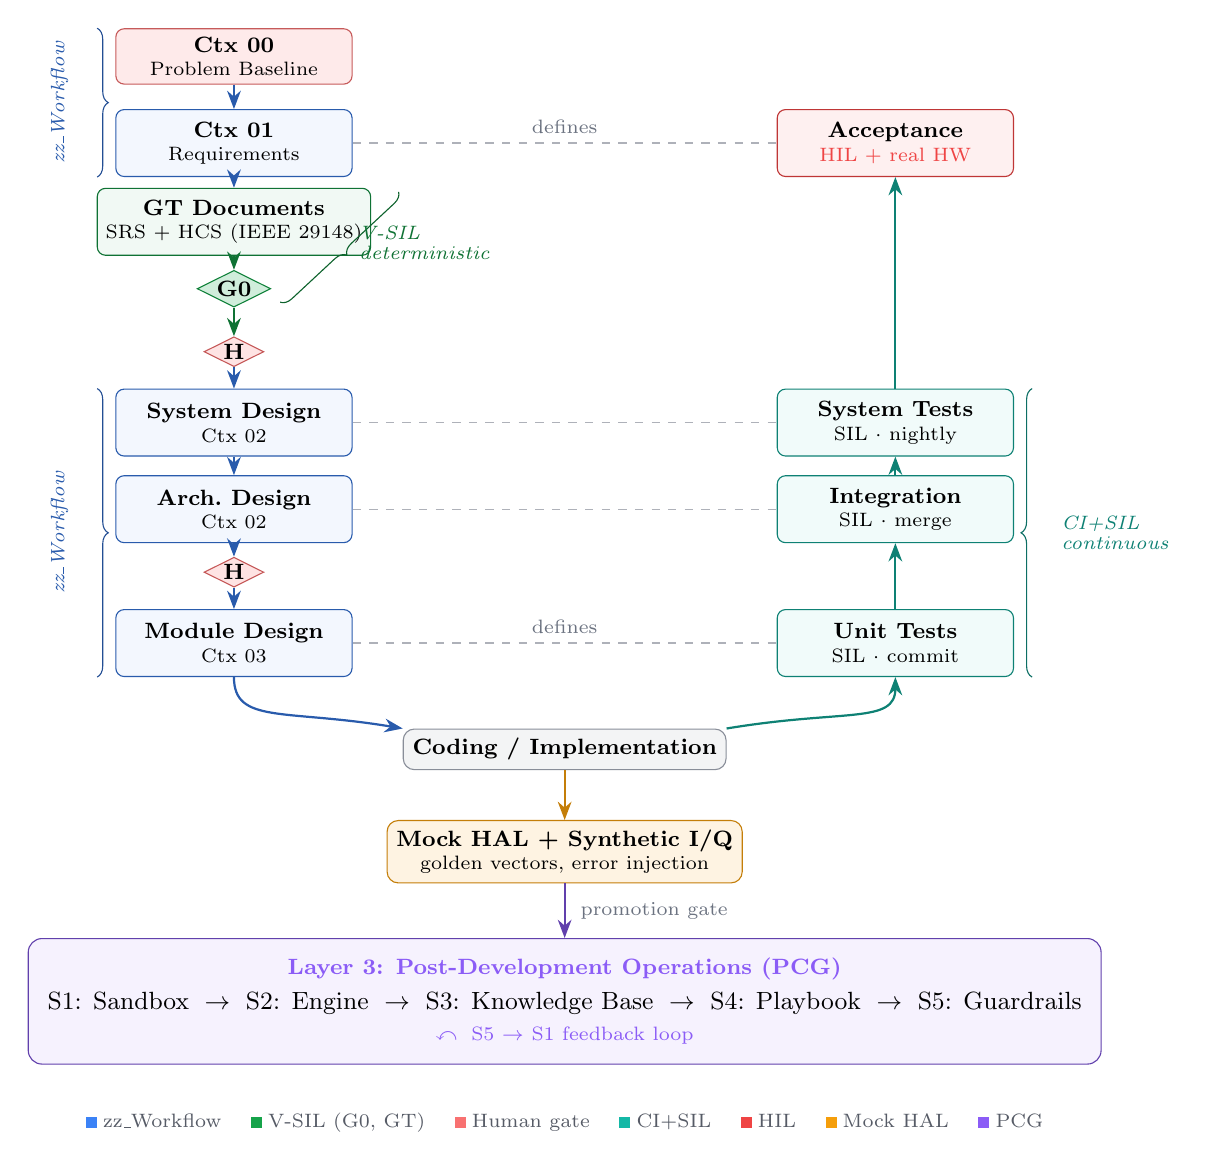
\begin{tikzpicture}[
  font=\footnotesize,
  >={Stealth[length=2.4mm]},
  % --- zz_Workflow styles (blue family) ---
  zzbox/.style={draw=zzblue!70!black, fill=zzblue!6, rounded corners=3pt,
                align=center, minimum width=30mm, minimum height=8.5mm, inner sep=3pt},
  zzgate/.style={draw=coral!80!black, fill=coral!20, diamond, aspect=2,
                 inner sep=0.5pt, font=\footnotesize\bfseries},
  zzflow/.style={draw=zzblue!70!black, thick, -{Stealth}},
  % --- V-SIL implementation styles (green family) ---
  vsbox/.style={draw=vsgreen!70!black, fill=vsgreen!6, rounded corners=3pt,
                align=center, minimum width=30mm, minimum height=8.5mm, inner sep=3pt},
  vsgate/.style={draw=vsgreen!80!black, fill=vsgreen!20, diamond, aspect=2,
                 inner sep=0.5pt, font=\footnotesize\bfseries},
  vsflow/.style={draw=vsgreen!70!black, thick, -{Stealth}},
  % --- CI+SIL styles (teal) ---
  cibox/.style={draw=vteal!70!black, fill=vteal!6, rounded corners=3pt,
                align=center, minimum width=30mm, minimum height=8.5mm, inner sep=3pt},
  ciflow/.style={draw=vteal!70!black, thick, -{Stealth}},
  % --- Shared ---
  hil/.style={cibox, draw=vred!80!black, fill=vred!8},
  def/.style={draw=vgrey!55, dashed, thin},
  brace/.style={decorate, decoration={brace, amplitude=4pt, raise=2pt}}
]

% ---- LEFT ARM (descending) ----
\node[draw=coral!80!black, fill=coral!15, rounded corners=3pt, align=center,
      minimum width=30mm, inner sep=3pt] (ctx00) at (-4.2,8.0)
      {\textbf{Ctx 00}\\[-1pt]{\scriptsize Problem Baseline}};

\node[zzbox] (l1L) at (-4.2,6.9) {\textbf{Ctx 01}\\[-1pt]{\scriptsize Requirements}};

\node[vsbox] (gt) at (-4.2,5.9)
      {\textbf{GT Documents}\\[-1pt]{\scriptsize SRS + HCS (IEEE 29148)}};
\node[vsgate] (g0) at (-4.2,5.05) {G0};

\node[zzgate] (g1)  at (-4.2,4.25) {H};
\node[zzbox] (l2L) at (-4.2,3.35) {\textbf{System Design}\\[-1pt]{\scriptsize Ctx 02}};
\node[zzbox] (l3L) at (-4.2,2.25) {\textbf{Arch.\ Design}\\[-1pt]{\scriptsize Ctx 02}};
\node[zzgate] (g2)  at (-4.2,1.45) {H};
\node[zzbox] (l4L) at (-4.2,0.55) {\textbf{Module Design}\\[-1pt]{\scriptsize Ctx 03}};

\draw[zzflow] (ctx00.south) -- (l1L.north);
\draw[zzflow] (l1L.south)   -- (gt.north);
\draw[vsflow] (gt.south)    -- (g0.north);
\draw[vsflow] (g0.south)    -- (g1.north);
\draw[zzflow] (g1.south)    -- (l2L.north);
\draw[zzflow] (l2L.south)   -- (l3L.north);
\draw[zzflow] (l3L.south)   -- (g2.north);
\draw[zzflow] (g2.south)    -- (l4L.north);

% ---- Side brackets ----
\draw[brace, zzblue!60!black] ([xshift=-3mm]ctx00.north west)
  -- ([xshift=-3mm]l1L.south west)
  node[midway, left=5pt, font=\scriptsize\itshape, text=zzblue!70!black,
       align=right, rotate=90, anchor=south] {zz\_Workflow};
\draw[brace, zzblue!60!black] ([xshift=-3mm]l2L.north west)
  -- ([xshift=-3mm]l4L.south west)
  node[midway, left=5pt, font=\scriptsize\itshape, text=zzblue!70!black,
       align=right, rotate=90, anchor=south] {zz\_Workflow};

\draw[brace, vsgreen!60!black] ([xshift=3mm]gt.north east)
  -- ([xshift=3mm]g0.south east)
  node[midway, right=5pt, font=\scriptsize\itshape, text=vsgreen!70!black,
       align=left] {V-SIL\\[-1pt]{\scriptsize deterministic}};

% ---- RIGHT ARM (ascending, CI+SIL) ----
\node[hil]  (l1R) at (4.2,6.9) {\textbf{Acceptance}\\[-1pt]
  {\scriptsize\color{vred}HIL + real HW}};
\node[cibox] (l2R) at (4.2,3.35) {\textbf{System Tests}\\[-1pt]
  {\scriptsize SIL $\cdot$ nightly}};
\node[cibox] (l3R) at (4.2,2.25) {\textbf{Integration}\\[-1pt]
  {\scriptsize SIL $\cdot$ merge}};
\node[cibox] (l4R) at (4.2,0.55) {\textbf{Unit Tests}\\[-1pt]
  {\scriptsize SIL $\cdot$ commit}};

\draw[ciflow] (l4R.north) -- (l3R.south);
\draw[ciflow] (l3R.north) -- (l2R.south);
\draw[ciflow] (l2R.north) -- (l1R.south);

\draw[brace, vteal!60!black] ([xshift=3mm]l4R.south east)
  -- ([xshift=3mm]l2R.north east)
  node[midway, right=5pt, font=\scriptsize\itshape, text=vteal!70!black,
       align=left] {CI+SIL\\[-1pt]{\scriptsize continuous}};

% ---- "defines" links ----
\draw[def] (l1L.east) -- (l1R.west)
  node[midway, above, font=\scriptsize, text=vgrey] {defines};
\draw[def] (l2L.east) -- (l2R.west);
\draw[def] (l3L.east) -- (l3R.west);
\draw[def] (l4L.east) -- (l4R.west)
  node[midway, above, font=\scriptsize, text=vgrey] {defines};

% ---- Valley + Mock HAL ----
\node[draw=vgrey!80, fill=vgrey!8, rounded corners=4pt, align=center,
      minimum width=32mm] (valley) at (0,-0.8)
      {\textbf{Coding / Implementation}};

\draw[zzflow] (l4L.south) .. controls ++(0,-0.6) and ++(-1.5,0.25) .. (valley.north west);
\draw[ciflow] (valley.north east) .. controls ++(1.5,0.25) and ++(0,-0.6) .. (l4R.south);

\node[draw=amber!80!black, fill=amber!12, rounded corners=4pt, align=center,
      minimum width=32mm] (mock) at (0,-2.1)
      {\textbf{Mock HAL + Synthetic I/Q}\\[-1pt]
       {\scriptsize golden vectors, error injection}};
\draw[draw=amber!80!black, thick, -{Stealth}] (valley.south) -- (mock.north);

% ---- PCG band (Layer 3) ----
\node[draw=violet!70!black, fill=violet!8, rounded corners=5pt, align=center,
      minimum width=11cm, inner sep=7pt] (pcg) at (0,-4.0)
      {\textbf{\color{violet}Layer 3: Post-Development Operations (PCG)}\\[3pt]
       {\small S1: Sandbox $\;\to\;$ S2: Engine $\;\to\;$ S3: Knowledge Base
       $\;\to\;$ S4: Playbook $\;\to\;$ S5: Guardrails}\\[2pt]
       {\scriptsize\color{violet}$\curvearrowleft$\; S5 $\to$ S1 feedback loop}};

\draw[draw=violet!70!black, thick, -{Stealth}] (mock.south) -- (pcg.north)
  node[midway, right=2pt, font=\scriptsize, text=vgrey] {promotion gate};

% ---- Legend ----
\node[anchor=north, font=\scriptsize, align=center, text=vgrey!80!black] at (0,-5.3) {%
  \textcolor{zzblue}{\rule{0.5em}{0.5em}}\;zz\_Workflow \quad
  \textcolor{vsgreen}{\rule{0.5em}{0.5em}}\;V-SIL (G0, GT) \quad
  \textcolor{coral}{\rule{0.5em}{0.5em}}\;Human gate \quad
  \textcolor{vteal}{\rule{0.5em}{0.5em}}\;CI+SIL \quad
  \textcolor{vred}{\rule{0.5em}{0.5em}}\;HIL \quad
  \textcolor{amber}{\rule{0.5em}{0.5em}}\;Mock HAL \quad
  \textcolor{violet}{\rule{0.5em}{0.5em}}\;PCG};

\end{tikzpicture}}%
\caption{\textbf{V-SIL lifecycle.} Blue: conceptual methodology (zz\_Workflow); green:
deterministic V-SIL additions (GT, Gate G0); coral: human readiness gates; teal: continuous
SIL test arm; red: the only HIL level; violet: post-development pipeline.}
\label{fig:vsil}
\end{figure}

\begin{table}[htbp]
\centering
\caption{The three layers and their terminal outputs.}
\label{tab:layers}
\small
\begin{tabular}{@{}clllp{4.0cm}@{}}
\toprule
\textbf{\#} & \textbf{Name} & \textbf{Source} & \textbf{Purpose} & \textbf{Terminal output} \\
\midrule
1 & Conceptual Validation & zz\_Workflow & Define and validate what to build & Verified Prototype + Evidence \\
2 & Software Development & CI+SIL & Implement and continuously verify & Regression-passing build \\
3 & Post-Development Ops & PCG & Govern the deployed system & Audit-ready evidence archive \\
\bottomrule
\end{tabular}
\end{table}

% ===========================================================================
\section{Gate G0 --- Structural Validation of Ground Truth}
% ===========================================================================

G0 is the first gate and the only fully implemented one: \textbf{no AI, pure script}
(\texttt{g0\_validate.py}, stdlib-only, no network, no writes). It answers one question ---
\emph{does each GT document follow the IEEE 29148 template?} --- in four phases, with a
binary verdict (exit 0 / exit 1). Errors block; warnings do not. A failure routes back to the
GT author (R1) before any human reviewer sees the document.

\begin{figure}[htbp]
\centering
\resizebox{0.78\textwidth}{!}{%
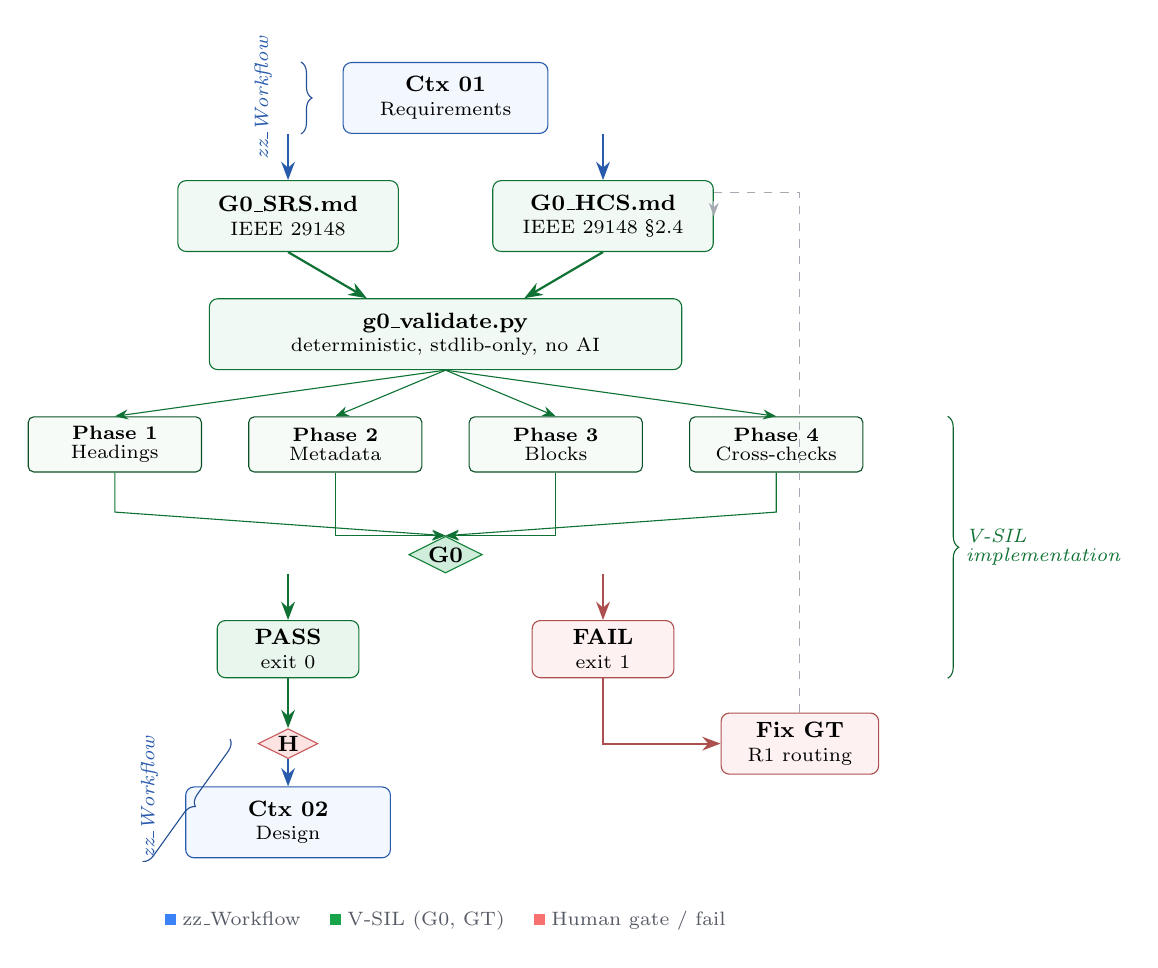
\begin{tikzpicture}[
  font=\footnotesize,
  >={Stealth[length=2.4mm]},
  zzn/.style={draw=zzblue!70!black, fill=zzblue!6, rounded corners=3pt,
              align=center, minimum width=26mm, minimum height=9mm, inner sep=3pt},
  zzarr/.style={draw=zzblue!70!black, thick, -{Stealth}},
  vsn/.style={draw=vsgreen!70!black, fill=vsgreen!6, rounded corners=3pt,
              align=center, minimum width=26mm, minimum height=9mm, inner sep=3pt},
  vsarr/.style={draw=vsgreen!70!black, thick, -{Stealth}},
  ph/.style={draw=vsgreen!50!black, fill=vsgreen!4, rounded corners=2pt,
             align=center, minimum width=22mm, minimum height=7mm,
             font=\scriptsize, inner sep=2pt},
  zzgate/.style={draw=coral!80!black, fill=coral!20, diamond, aspect=2,
                 inner sep=0.5pt, font=\footnotesize\bfseries},
  vsgate/.style={draw=vsgreen!80!black, fill=vsgreen!20, diamond, aspect=2,
                 inner sep=0.5pt, font=\footnotesize\bfseries},
  pass/.style={draw=vsgreen!70!black, fill=vsgreen!10, rounded corners=3pt,
               align=center, minimum width=18mm, font=\footnotesize},
  fail/.style={draw=coral!70!black, fill=coral!10, rounded corners=3pt,
               align=center, minimum width=18mm, font=\footnotesize},
  fb/.style={draw=vgrey!60, dashed, -{Stealth}, thin},
  brace/.style={decorate, decoration={brace, amplitude=4pt, raise=2pt}}
]

% ---- Ctx 01 -> GT ----
\node[zzn] (ctx01) at (0,0) {\textbf{Ctx 01}\\[-1pt]{\scriptsize Requirements}};

\node[vsn, minimum width=28mm] (srs) at (-2,-1.5)
      {\textbf{G0\_SRS.md}\\[-1pt]{\scriptsize IEEE 29148}};
\node[vsn, minimum width=28mm] (hcs) at ( 2,-1.5)
      {\textbf{G0\_HCS.md}\\[-1pt]{\scriptsize IEEE 29148 \S2.4}};
\draw[zzarr] (ctx01.south -| srs.north) -- (srs.north);
\draw[zzarr] (ctx01.south -| hcs.north) -- (hcs.north);

% ---- Validator ----
\node[vsn, minimum width=60mm] (g0v) at (0,-3)
      {\textbf{g0\_validate.py}\\[-1pt]{\scriptsize deterministic, stdlib-only, no AI}};
\draw[vsarr] (srs.south) -- ([xshift=-10mm]g0v.north);
\draw[vsarr] (hcs.south) -- ([xshift= 10mm]g0v.north);

% ---- 4 phases ----
\node[ph] (p1) at (-4.2,-4.4) {\textbf{Phase 1}\\[-1pt]Headings};
\node[ph] (p2) at (-1.4,-4.4) {\textbf{Phase 2}\\[-1pt]Metadata};
\node[ph] (p3) at ( 1.4,-4.4) {\textbf{Phase 3}\\[-1pt]Blocks};
\node[ph] (p4) at ( 4.2,-4.4) {\textbf{Phase 4}\\[-1pt]Cross-checks};
\foreach \p in {p1,p2,p3,p4}{
  \draw[vsarr, thin] (g0v.south) -- (\p.north);
}

% ---- Verdict ----
\node[vsgate] (verdict) at (0,-5.8) {G0};
\draw[vsarr, thin] (p1.south) |- ([yshift=3mm]verdict.north -| p1) -- (verdict.north);
\draw[vsarr, thin] (p2.south) -- (verdict.north -| p2) -- (verdict.north);
\draw[vsarr, thin] (p3.south) -- (verdict.north -| p3) -- (verdict.north);
\draw[vsarr, thin] (p4.south) |- ([yshift=3mm]verdict.north -| p4) -- (verdict.north);

% ---- Pass / Fail ----
\node[pass] (ok) at (-2,-7) {\textbf{PASS}\\[-1pt]{\scriptsize exit 0}};
\node[fail] (ko) at ( 2,-7) {\textbf{FAIL}\\[-1pt]{\scriptsize exit 1}};
\draw[vsarr] (verdict.south -| ok) -- (ok.north);
\draw[draw=coral!70!black, thick, -{Stealth}] (verdict.south -| ko) -- (ko.north);

% ---- Downstream ----
\node[zzgate] (gateH) at (-2,-8.2) {H};
\draw[vsarr] (ok.south) -- (gateH.north);

\node[zzn, minimum width=26mm] (ctx02) at (-2,-9.2)
      {\textbf{Ctx 02}\\[-1pt]{\scriptsize Design}};
\draw[zzarr] (gateH.south) -- (ctx02.north);

% ---- Fail feedback ----
\node[fail, minimum width=20mm] (fix) at (4.5,-8.2)
      {\textbf{Fix GT}\\[-1pt]{\scriptsize R1 routing}};
\draw[draw=coral!70!black, thick, -{Stealth}] (ko.south) |- (fix.west);
\draw[fb] (fix.north) |- ([yshift=3mm]hcs.east) -- (hcs.east);

% ---- Side brackets ----
\draw[brace, vsgreen!60!black] ([xshift=10mm]p4.north east)
  -- ([xshift=10mm]p4.north east |- ko.south)
  node[midway, right=5pt, font=\scriptsize\itshape, text=vsgreen!70!black,
       align=left] {V-SIL\\[-1pt]{\scriptsize implementation}};

\draw[brace, zzblue!60!black] ([xshift=-6mm]ctx01.north west)
  -- ([xshift=-6mm]ctx01.south west)
  node[midway, left=5pt, font=\scriptsize\itshape, text=zzblue!70!black,
       rotate=90, anchor=south] {zz\_Workflow};
\draw[brace, zzblue!60!black] ([xshift=-6mm]gateH.north west)
  -- ([xshift=-6mm]ctx02.south west)
  node[midway, left=5pt, font=\scriptsize\itshape, text=zzblue!70!black,
       rotate=90, anchor=south] {zz\_Workflow};

% ---- Legend ----
\node[anchor=north, font=\scriptsize, align=center, text=vgrey!80!black] at (0,-10.2) {%
  \textcolor{zzblue}{\rule{0.5em}{0.5em}}\;zz\_Workflow \quad
  \textcolor{vsgreen}{\rule{0.5em}{0.5em}}\;V-SIL (G0, GT) \quad
  \textcolor{coral}{\rule{0.5em}{0.5em}}\;Human gate / fail};

\end{tikzpicture}}%
\caption{\textbf{G0 validation flow.} Ctx 01 produces the GT documents; the script validates
them deterministically through four phases. PASS admits them to human Gate H and Ctx 02;
FAIL returns to fix the GT structure (R1). No AI is involved.}
\label{fig:g0flow}
\end{figure}

\begin{table}[htbp]
\centering
\caption{The four G0 validation phases.}
\label{tab:g0phases}
\small
\setlength{\tabcolsep}{5pt}
\begin{tabular}{@{}clp{8.6cm}@{}}
\toprule
\textbf{Phase} & \textbf{Target} & \textbf{Checks} \\
\midrule
1 & Document headings & All required headings present (substring match on normalized text) \\
2 & Metadata table & Document ID, Project, Organization, SemVer version, Classification --- no placeholders \\
3 & Blocks & ID format + uniqueness, required fields, enumerated types, description, $\geq 1$ acceptance criterion \\
4 & Cross-checks & SRS: traceability coverage + acyclic dependencies; HCS: no orphan components \\
\bottomrule
\end{tabular}
\end{table}

% ===========================================================================
\section{Gate G1 --- Ctx 02 Design Synthesis (GT $\to$ Architecture)}
% ===========================================================================

\begin{center}\footnotesize
\texttt{Ctx 00 $\to$ Ctx 01 $\to$ G0 \checkmark $\to$ [Ctx 02 \textbullet\ G1]
$\to$ Gate H $\to$ Ctx 03}
\end{center}

\vspace{-2pt}

G1 turns the validated GT into a software architecture. No single framework covers the Ctx 02
mandate, so G1 hybrids three: \textcolor{zzblue}{MAAD} (multi-hypothesis generation),
\textcolor{violet}{ARLO} (quantitative selection), and \textcolor{vteal}{ADD} (module
decomposition) --- closing with a human Gate H package.

\begin{figure}[htbp]
\centering
\resizebox{0.97\textwidth}{!}{%
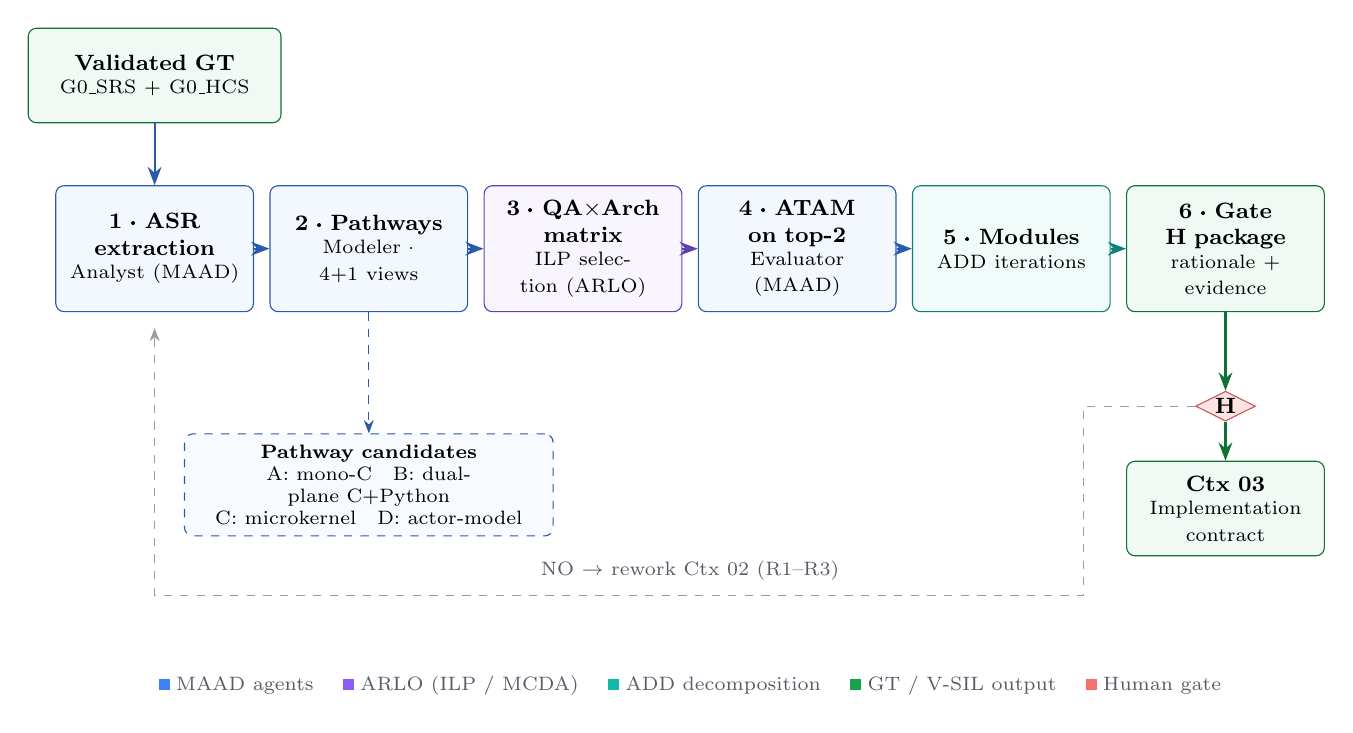
\begin{tikzpicture}[
  font=\footnotesize,
  >={Stealth[length=2.4mm]},
  block/.style={draw=#1!70!black, fill=#1!6, rounded corners=3pt, align=center,
                minimum width=2.5cm, text width=2.3cm, minimum height=1.6cm,
                inner sep=3pt},
  flow/.style={draw=#1!70!black, thick, -{Stealth}},
  gateh/.style={draw=coral!80!black, fill=coral!20, diamond, aspect=2,
                inner sep=0.5pt, font=\footnotesize\bfseries},
  fb/.style={draw=vgrey!70, dashed, thin, -{Stealth}}
]

% ---- Input: validated GT ----
\node[block=vsgreen, minimum width=3.2cm, text width=3.0cm, minimum height=1.2cm]
  (gt) at (-6.8,0.5)
  {\textbf{Validated GT}\\[-1pt]{\scriptsize G0\_SRS + G0\_HCS}};

% ---- Six steps ----
\node[block=zzblue] (s1) at (-6.8,-1.7)
  {\textbf{1 · ASR extraction}\\[-1pt]{\scriptsize Analyst (MAAD)}};
\node[block=zzblue] (s2) at (-4.08,-1.7)
  {\textbf{2 · Pathways}\\[-1pt]{\scriptsize Modeler · 4+1 views}};
\node[block=violet] (s3) at (-1.36,-1.7)
  {\textbf{3 · QA$\times$Arch matrix}\\[-1pt]{\scriptsize ILP selection (ARLO)}};
\node[block=zzblue] (s4) at (1.36,-1.7)
  {\textbf{4 · ATAM on top-2}\\[-1pt]{\scriptsize Evaluator (MAAD)}};
\node[block=vteal]  (s5) at (4.08,-1.7)
  {\textbf{5 · Modules}\\[-1pt]{\scriptsize ADD iterations}};
\node[block=vsgreen] (s6) at (6.8,-1.7)
  {\textbf{6 · Gate H package}\\[-1pt]{\scriptsize rationale + evidence}};

\draw[flow=zzblue] (gt.south)  -- (s1.north);
\draw[flow=zzblue] (s1.east) -- (s2.west);
\draw[flow=zzblue] (s2.east) -- (s3.west);
\draw[flow=violet] (s3.east) -- (s4.west);
\draw[flow=zzblue] (s4.east) -- (s5.west);
\draw[flow=vteal]  (s5.east) -- (s6.west);

% ---- Candidate pathways (under step 2) ----
\node[draw=zzblue!70!black, fill=zzblue!4, dashed, rounded corners=3pt, align=center,
      text width=4.4cm, font=\scriptsize, inner sep=4pt] (pw) at (-4.08,-4.7)
  {\textbf{Pathway candidates}\\
   A: mono-C \; B: dual-plane C+Python\\
   C: microkernel \; D: actor-model};
\draw[draw=zzblue!70!black, thin, dashed, -{Stealth}] (s2.south) -- (pw.north);

% ---- Human Gate H -> Ctx 03 ----
\node[gateh] (h) at (6.8,-3.7) {H};
\draw[draw=vsgreen!70!black, thick, -{Stealth}] (s6.south) -- (h.north);

\node[block=vsgreen, minimum height=1.2cm] (ctx03) at (6.8,-5.0)
  {\textbf{Ctx 03}\\[-1pt]{\scriptsize Implementation contract}};
\draw[draw=vsgreen!70!black, thick, -{Stealth}] (h.south) -- (ctx03.north);

% ---- Feedback: Gate H NO -> rework (R1-R3) ----
\draw[fb] (h.west) -- (5.0,-3.7) -- (5.0,-6.1) -- (-6.8,-6.1)
  -- ([yshift=-2mm]s1.south);
\node[anchor=south, yshift=2pt, font=\scriptsize, text=vgrey!80!black] at (0,-6.1)
  {NO $\to$ rework Ctx 02 (R1--R3)};

% ---- Legend ----
\node[anchor=north, font=\scriptsize, text=vgrey!80!black] at (0,-7.0) {%
  \textcolor{zzblue}{\rule{0.5em}{0.5em}}\;MAAD agents \quad
  \textcolor{violet}{\rule{0.5em}{0.5em}}\;ARLO (ILP / MCDA) \quad
  \textcolor{vteal}{\rule{0.5em}{0.5em}}\;ADD decomposition \quad
  \textcolor{vsgreen}{\rule{0.5em}{0.5em}}\;GT / V-SIL output \quad
  \textcolor{coral}{\rule{0.5em}{0.5em}}\;Human gate};

\end{tikzpicture}}%
\caption{\textbf{G1 design pipeline (hybrid MAAD + ARLO + ADD).} The validated GT feeds
six steps: extract architecturally significant requirements, generate 3--4 candidate
pathways with 4+1 views, score them in a QA$\times$architecture matrix solved by ILP, run
ATAM on the top two, decompose the winner into modules, and package everything for human
Gate H. A NO routes defects back into the stage (R1--R3).}
\label{fig:g1design}
\end{figure}

\begin{table}[htbp]
\centering
\caption{Why G1 hybrids four frameworks: none covers Ctx 02 alone.}
\label{tab:frameworks}
\scriptsize
\setlength{\tabcolsep}{4pt}
\begin{tabular}{@{}lp{3.1cm}p{3.1cm}p{3.1cm}p{3.1cm}@{}}
\toprule
\textbf{Criterion} & \textbf{MAAD} & \textbf{ARLO} & \textbf{ADD+LLM} & \textbf{SDD} \\
\midrule
Multi-hypothesis & Native (mismatch report) & Native (ILP candidates) & Needs adaptation & No \\
Module decomposition & 4+1 views $\to$ components & Style only, no modules & Fine-grained per iteration & Contract-level only \\
Quantitative selection & Qualitative ATAM & ILP optimization (MCDA) & Implicit & N/A \\
HW-constraint support & Via RAG injection & Via QA mapping & Via driver ID & Via spec contracts \\
Trade-study output & Sensitivity / risk catalog & Scored matrix + solution & Pattern rationale & Pass/fail per contract \\
Ctx 02 coverage & Full & Selection only & Decomposition only & Verification only \\
\bottomrule
\end{tabular}
\end{table}

\end{document}
